\section{Thiết kế hệ thống}
\subsection{Useccase Diagram toàn hệ thống}
\begin{figure} [H]
    \centering
    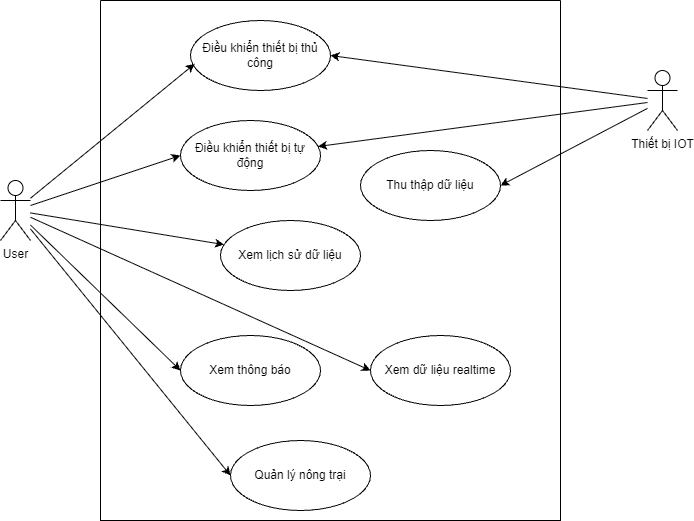
\includegraphics[width=0.8\textwidth]{img/sodousecase.png}
    \caption{Usecase Diagram toàn hệ thống}
\end{figure}

\newcolumntype{L}{>{\RaggedRight\arraybackslash}p{0.24\textwidth}}
\newcolumntype{R}{>{\RaggedRight\arraybackslash}p{0.70\textwidth}}

% =========================================================
\subsection{Điều khiển thiết bị thủ công}
% =========================================================
 
\begin{longtable}{|L|R|}
 
\hline
\textbf{Trường} & \textbf{Nội dung} \\ \hline
 
\endfirsthead
 
\hline
\textbf{Trường} & \textbf{Nội dung} \\ \hline
 
\endhead
 
\endfoot
 
Tên Usecase & Điều khiển thiết bị thủ công \\[4pt] \hline
 
Tác nhân & Người dùng, Thiết bị IOT \\[4pt] \hline
 
Mô tả & Cho phép người dùng điều khiển thiết bị một cách thủ công (máy bơm). \\[4pt] \hline
 
Tiền điều kiện &
\begin{itemize}[leftmargin=*, nosep, topsep=2pt]
  \item Người dùng đã đăng nhập vào hệ thống và đã chọn nông trại quản lý.
  \item Thiết bị IOT hoạt động bình thường.
  \item Kết nối mạng giữa các thiết bị IOT và hệ thống duy trì ổn định.
\end{itemize} \\[4pt] \hline
 
Hậu điều kiện & Thiết bị được điều khiển thủ công từ người dùng. \\[4pt] \hline
 
Luồng cơ bản &
\begin{enumerate}[leftmargin=*, nosep, topsep=2pt]
  \item Người dùng đã chọn nông trại cần quản lý.
  \item Người dùng chọn máy bơm muốn điều khiển.
  \item Người dùng bật/tắt thiết bị.
  \item Hệ thống gửi dữ liệu và kích hoạt thiết bị thành công.
  \item Hệ thống cập nhật trạng thái mới của thiết bị cho người dùng.
\end{enumerate} \\[4pt] \hline
 
Luồng thay thế &
\textit{Ngoại lệ 1:} Thiết bị không nhận được dữ liệu do mạng hoặc phần cứng.
Hệ thống thông báo lỗi và yêu cầu thử lại. \\[4pt] \hline
 
\end{longtable}
 
% =========================================================
\subsection{Điều khiển thiết bị tự động}
% =========================================================
 
\begin{longtable}{|L|R|}
 
\hline
\textbf{Trường} & \textbf{Nội dung} \\ \hline
 
\endfirsthead
 
\hline
\textbf{Trường} & \textbf{Nội dung} \\ \hline
 
\endhead
 
\endfoot
 
Tên Usecase & Điều khiển thiết bị tự động \\[4pt] \hline
 
Tác nhân & Người dùng, Thiết bị IOT \\[4pt] \hline
 
Mô tả & Cho phép người dùng điều khiển thiết bị một cách tự động (máy bơm). \\[4pt] \hline
 
Tiền điều kiện &
\begin{itemize}[leftmargin=*, nosep, topsep=2pt]
  \item Người dùng đã đăng nhập vào hệ thống và đã chọn nông trại quản lý.
  \item Thiết bị IOT hoạt động bình thường.
  \item Kết nối mạng giữa các thiết bị IOT và hệ thống duy trì ổn định.
\end{itemize} \\[4pt] \hline
 
Hậu điều kiện & Thiết bị hoạt động tự động theo cài đặt của người dùng. \\[4pt] \hline
 
Luồng cơ bản &
\begin{enumerate}[leftmargin=*, nosep, topsep=2pt]
  \item Người dùng đã chọn nông trại cần quản lý.
  \item Người dùng chọn máy bơm muốn điều khiển.
  \item Hệ thống hiển thị giao diện cài đặt thời gian tự động.
  \item Người dùng chọn giờ bật, tắt, các thông tin khác.
  \item Hệ thống kiểm tra thông tin.
  \item Hệ thống thông báo cập nhật thành công.
\end{enumerate} \\[4pt] \hline
 
Luồng thay thế &
\begin{itemize}[leftmargin=*, nosep, topsep=2pt]
  \item \textit{Ngoại lệ 1:} Thiết bị không nhận được dữ liệu do mạng hoặc phần cứng. Hệ thống thông báo lỗi và yêu cầu thử lại.
  \item \textit{Ngoại lệ 2:} Thời gian không hợp lệ. Hệ thống thông báo lỗi và yêu cầu thử lại.
  \item \textit{Ngoại lệ 3:} Điều chỉnh theo độ ẩm đất. Hệ thống hiển thị giao diện nhập ngưỡng độ ẩm bật/tắt thiết bị. Người dùng nhập đầy đủ dữ liệu. Hệ thống kiểm tra dữ liệu. Hệ thống thông báo cập nhật thành công.
\end{itemize} \\[4pt] \hline
 
\end{longtable}

\subsection{Xem dữ liệu realtime}
% =========================================================
 
\begin{longtable}{|L|R|}
 
\hline
\textbf{Trường} & \textbf{Nội dung} \\ \hline
 
\endfirsthead
 
\hline
\textbf{Trường} & \textbf{Nội dung} \\ \hline
 
\endhead
 
\endfoot
 
Tên Usecase & Xem dữ liệu realtime \\[4pt] \hline
 
Tác nhân & Người dùng \\[4pt] \hline
 
Mô tả & Người dùng có thể xem dữ liệu cảm biến (nhiệt độ, độ ẩm không khí, độ ẩm đất, ánh sáng) theo thời gian thực trên ứng dụng. \\[4pt] \hline
 
Tiền điều kiện &
\begin{itemize}[leftmargin=*, nosep, topsep=2pt]
  \item Người dùng đã đăng nhập vào hệ thống và đã chọn nông trại quản lý.
  \item Các cảm biến hoạt động bình thường và đang gửi dữ liệu lên hệ thống.
  \item Kết nối mạng giữa các thiết bị IOT và hệ thống duy trì ổn định.
\end{itemize} \\[4pt] \hline
 
Hậu điều kiện &
\begin{itemize}[leftmargin=*, nosep, topsep=2pt]
  \item Dữ liệu môi trường (nhiệt độ, độ ẩm, trạng thái máy bơm) hiển thị chính xác trên giao diện người dùng.
  \item Hệ thống cập nhật dữ liệu mới nhất theo thời gian thực.
  \item Nếu có bất thường về dữ liệu, hệ thống sẽ gửi cảnh báo.
\end{itemize} \\[4pt] \hline
 
Luồng cơ bản &
\begin{enumerate}[leftmargin=*, nosep, topsep=2pt]
  \item Người dùng đã chọn nông trại cần quản lý.
  \item Hệ thống lấy dữ liệu từ Adafruit IO.
  \item Adafruit IO phản hồi dữ liệu cảm biến về backend.
  \item Hệ thống hiển thị các thông số: Nhiệt độ, độ ẩm không khí, độ ẩm đất, ánh sáng theo thời gian thực.
  \item Hệ thống lưu trữ dữ liệu vào cơ sở dữ liệu kèm theo thời gian để phục vụ hiển thị báo cáo sau này.
\end{enumerate} \\[4pt] \hline
 
Luồng thay thế &
\textit{Ngoại lệ:} Không lấy được dữ liệu do mạng, phần cứng hoặc lỗi khác.
Hệ thống hiển thị thông báo lỗi và yêu cầu thử lại sau. \\[4pt] \hline
 
\end{longtable}
 
% =========================================================
\subsection{Xem lịch sử dữ liệu}
% =========================================================
 
\begin{longtable}{|L|R|}
 
\hline
\textbf{Trường} & \textbf{Nội dung} \\ \hline
 
\endfirsthead
 
\hline
\textbf{Trường} & \textbf{Nội dung} \\ \hline
 
\endhead
 
\endfoot
 
Tên Usecase & Xem lịch sử dữ liệu \\[4pt] \hline
 
Tác nhân & Người dùng \\[4pt] \hline
 
Mô tả & Người dùng có thể xem lịch sử dữ liệu từ cảm biến bao gồm nhiệt độ, độ ẩm không khí, ánh sáng trong 12 giờ, 7 ngày, 30 ngày gần nhất. \\[4pt] \hline
 
Tiền điều kiện &
\begin{itemize}[leftmargin=*, nosep, topsep=2pt]
  \item Người dùng đã đăng nhập vào hệ thống và đã chọn nông trại quản lý.
  \item Dữ liệu được lưu vào cơ sở dữ liệu thường xuyên.
\end{itemize} \\[4pt] \hline
 
Hậu điều kiện & Hệ thống hiển thị lịch sử thông tin dữ liệu theo dạng biểu đồ. \\[4pt] \hline
 
Luồng cơ bản &
\begin{enumerate}[leftmargin=*, nosep, topsep=2pt]
  \item Người dùng đã chọn nông trại cần quản lý.
  \item Người dùng chọn chức năng lịch sử và chọn dữ liệu muốn xem.
  \item Hệ thống cập nhật dữ liệu từ cơ sở dữ liệu và hiển thị ra màn hình.
  \item Người dùng chọn vào các điểm trên biểu đồ để xem chi tiết dữ liệu tại thời gian cụ thể.
  \item Hệ thống hiển thị dữ liệu kèm thời gian cụ thể.
\end{enumerate} \\[4pt] \hline
 
Luồng thay thế &
\textit{Tại bước 4:} Người dùng chọn mức thời gian khác (24 giờ, 7 ngày, 30 ngày).
Hệ thống hiển thị lại biểu đồ biểu diễn dữ liệu tương ứng. \\[4pt] \hline
 
\end{longtable}
 
% =========================================================
\subsection{Quản lý nông trại}
% =========================================================
 
\begin{longtable}{|L|R|}
 
\hline
\textbf{Trường} & \textbf{Nội dung} \\ \hline
 
\endfirsthead
 
\hline
\textbf{Trường} & \textbf{Nội dung} \\ \hline
 
\endhead
 
\endfoot
 
Tên Usecase & Quản lý nông trại \\[4pt] \hline
 
Tác nhân & Người dùng \\[4pt] \hline
 
Mô tả & Người dùng chọn một nông trại bất kỳ trong danh sách để thực hiện các thao tác. \\[4pt] \hline
 
Tiền điều kiện & Người dùng đã đăng nhập vào hệ thống. \\[4pt] \hline
 
Hậu điều kiện & Hệ thống hiển thị các thông tin và chức năng để quản lý nông trại đó. \\[4pt] \hline
 
Luồng cơ bản &
\begin{enumerate}[leftmargin=*, nosep, topsep=2pt]
  \item Người dùng đăng nhập vào hệ thống.
  \item Hệ thống hiển thị danh sách nông trại hiện có.
  \item Người dùng chọn một nông trại muốn quản lý.
  \item Hệ thống hiển thị giao diện quản lý nông trại đó.
  \item Người dùng thực hiện các thao tác trên nông trại.
\end{enumerate} \\[4pt] \hline
 
Luồng thay thế &
\textit{Ngoại lệ:} Hệ thống không thể tải được dữ liệu.
Hệ thống hiển thị thông báo lỗi và yêu cầu thử lại sau. \\[4pt] \hline
 
\end{longtable}
 
% =========================================================
\subsection{Xem thông báo}
% =========================================================
 
\begin{longtable}{|L|R|}
 
\hline
\textbf{Trường} & \textbf{Nội dung} \\ \hline
 
\endfirsthead
 
\hline
\textbf{Trường} & \textbf{Nội dung} \\ \hline
 
\endhead
 
\endfoot
 
Tên Usecase & Xem thông báo \\[4pt] \hline
 
Tác nhân & Người dùng \\[4pt] \hline
 
Mô tả & Cho phép người dùng xem các thông báo cảnh báo quá mức của dữ liệu và trạng thái của nông trại. \\[4pt] \hline
 
Tiền điều kiện &
\begin{itemize}[leftmargin=*, nosep, topsep=2pt]
  \item Người dùng đã đăng nhập vào hệ thống và đã chọn nông trại quản lý.
  \item Dữ liệu được lưu vào cơ sở dữ liệu thường xuyên.
\end{itemize} \\[4pt] \hline
 
Hậu điều kiện & Hệ thống hiển thị các thông báo quá ngưỡng của dữ liệu (độ ẩm đất, nhiệt độ, độ ẩm không khí). \\[4pt] \hline
 
Luồng cơ bản &
\begin{enumerate}[leftmargin=*, nosep, topsep=2pt]
  \item Người dùng đã chọn nông trại cần quản lý.
  \item Người dùng chọn chức năng thông báo.
  \item Hệ thống hiển thị thông báo mới và lịch sử nhật ký các biến động trên nông trại.
\end{enumerate} \\[4pt] \hline
 
Luồng thay thế &
\textit{Ngoại lệ:} Hệ thống không thể tải được dữ liệu.
Hệ thống hiển thị thông báo lỗi và yêu cầu thử lại sau. \\[4pt] \hline
 
\end{longtable}
 